\documentclass[12pt,a4paper]{scrreprt}
\usepackage[utf8]{inputenc}
\usepackage{natbib}
\usepackage{colortbl}
\usepackage{listings}
\usepackage{booktabs}
\usepackage{subfigure}
\usepackage{tikz}
\usepackage{color}
\usepackage[plainpages=false,pdfpagelabels,bookmarks]{hyperref}
\hypersetup{
  pdftitle={Discourse Network Analyzer (DNA) - Documentation},
  pdfauthor={Philip Leifeld},
  pdfkeywords={DNA, discourse networks, Discourse Network Analyzer, social network analysis, SNA, policy networks, advocacy coalitions},
  pdfsubject={http://www.philipleifeld.de},
  breaklinks=true,
  colorlinks=true,
  urlcolor=darkblue,
  linkcolor=darkblue,
  citecolor=darkred,
  bookmarksnumbered
}

\bibpunct[: ]{(}{)}{;}{a}{}{,}

\emergencystretch 1.5em
\widowpenalty=10000
\clubpenalty=10000
\raggedbottom

\definecolor{darkred}{rgb}{0.9,0.1,0.1}
\definecolor{darkblue}{rgb}{0.1,0.1,0.9}
\definecolor{lightgray}{rgb}{0.92,0.92,0.92}

% Software-Logos
\newcommand{\visonecolor}
{\textsf%
 {\protect\raisebox{.5ex}{\color[rgb]{1,0,0}v}% red
  \protect\raisebox{.1ex}{\color[rgb]{0,1,0}i}% green
  \protect\raisebox{-.1ex}{\color[rgb]{0,0,1}s}% blue
  \protect\raisebox{.1ex}{\color[rgb]{1,0.8,0}o}% yellow
  \protect\raisebox{-.1ex}{\color[rgb]{1,0,0.8}n}% violet
  \protect\raisebox{-.4ex}{\color[rgb]{0,0.8,0.8}e}% cyan
 }%
}
\newcommand{\visone}
{\textsf%
 {\protect\raisebox{.5ex}{\color[rgb]{0.1,0.1,0.1}v}% dark gray
  \protect\raisebox{.1ex}{\color[rgb]{0.3,0.3,0.3}i}% light gray
  \protect\raisebox{-.1ex}{\color[rgb]{0.1,0.1,0.1}s}% dark gray
  \protect\raisebox{.1ex}{\color[rgb]{0.3,0.3,0.3}o}% light gray
  \protect\raisebox{-.1ex}{\color[rgb]{0.1,0.1,0.1}n}% dark gray
  \protect\raisebox{-.4ex}{\color[rgb]{0.3,0.3,0.3}e}% light gray
 }%
}
\newcommand{\ucinet}{\textsc{Ucinet}}
\newcommand{\netdraw}{\textsc{NetDraw}}
\newcommand{\R}{\textsc{R}}
\newcommand{\spss}{\textsc{Spss}}
\newcommand{\stata}{\textsc{Stata}}
\newcommand{\corel}{\textsc{CorelDraw}}
\newcommand{\excel}{\textsc{Excel}}
\newcommand{\calc}{\textsc{OpenOffice}.org \textsc{Calc}}
\newcommand{\automap}{\textsc{AutoMap}}
\newcommand{\vbpro}{\textsc{VB-Pro}}
\newcommand{\fulltext}{\textsc{Fulltext.exe}}
\newcommand{\inet}{\textsc{iNet}}
\newcommand{\dnalong}{\textsc{Discourse} \textsc{Network} \textsc{Analyzer}}
\newcommand{\dnashort}{\textsc{DNA}}
\newcommand{\commetrix}{\textsc{Commetrix}}
\newcommand{\sonia}{SoNIA}
\newcommand{\netminer}{\textsc{NetMiner}}
\newcommand{\gephi}{\textsc{Gephi}}

\newcommand{\code}[1]{\texttt{#1}}

\author{Philip Leifeld\footnote{Max Planck Institute for Research on Collective Goods, Kurt-Schumacher-Str.~10, 53113 Bonn, Germany | \href{mailto:Leifeld@coll.mpg.de}{\texttt{Leifeld@coll.mpg.de}} | \url{http://www.philipleifeld.de}}}
\title{
\includegraphics[width=2cm]{dna32.pdf}\\ \vspace{0.5cm} Discourse Network Analyzer (DNA)\\ \vspace{0.3cm} \textbf{Manual}}
\date{\today\\ \vspace{0.3cm} (valid for version 1.26)}

\begin{document}
\maketitle
\setcounter{tocdepth}{2}
\tableofcontents

\chapter{Introduction}
\dnalong\ (\dnashort) is a Java-based software for qualitative, category-based content analysis (QDA) with a special emphasis on the extraction of quantitative network data. Its main purpose is the actor-based analysis of political discourses. Yet it may be used for other applications or paradigms.

\dnashort\ involves two steps: coding statements of actors into categories, and converting these structured data into networks that are readable by \ucinet, \visone, \netminer, \gephi\ and other network-analytic software packages. The software can extract either bipartite (affiliation) networks or adjacency networks.

It is complementary to semantic network analysis applications because it neither relies on algorithms for automatic text processing, nor does it focus on the internal meaning or mental representation of a single text or document. Instead, tags are applied to the text data by manual inspection, thus rendering it more flexible, yet at the same time more work-intensive. \dnashort\ can be used to code a large body of text documents and then convert them into graphs.

More information about the software can be found in \citet{leifeld2009die,leifeld2010political} and \citet{leifeld2010comparison}. The underlying conceptual model is elaborated in the book chapter of \citet{janning2009diskursnetzwerkanalyse.}. The beginner's tutorial in chapter~\ref{demo} is based on empirical data collected by \citet{fisher2009understanding}.

If you would like to be informed about updates, please subscribe to the [DNA-help] mailing list at \url{http://www.philipleifeld.de}.


\chapter{Installation}\label{installation}
First, download the most recent version of the \dnalong\ from \url{http://www.philipleifeld.de}. Then make sure you have a recent version of the Java Runtime Engine (JRE) installed. Recent means version 1.6 or newer. If this is not the case, please download the newest Java version from \url{http://www.java.com}. Please do not try to run \dnashort\ with an older Java version because some important features will not work properly. \dnalong\ has been tested on Windows XP (SP\,1), Windows Vista, Windows 7, Ubuntu Linux 10.4, MacOS Leopard and MacOS Snow Leopard. However, it should work on any other operating system for which Java is available. Please check the FAQ in section~\ref{faq} if you encounter problems.

Some Java installations offer to start the software via double-clicking the file or right-clicking and selecting an entry from the context menu. However, the preferred way of starting \dnashort\ is from the command line by executing the command \code{java -jar dna-1.xx.jar} (where \code{xx} should be replaced by the current version number) from the folder where you have saved the file.

On Windows XP, you can do this as follows: Save the current version of DNA on your desktop. Go to the start menu and click on \code{Run}. A small window will pop up. Enter \code{cmd} into the text field of the window and press enter. A black window with the command line will be opened. Enter \code{cd Desktop} and press enter. Enter \code{java -jar dna-1.xx.jar} (replace \code{xx} by the current version number!) and press enter. DNA will now be loaded.

On Unix-based machines, you should be able to use the same command on the shell to start \dnashort.

Do not close the command line window because it will display important messages and possibly warnings or error messages. If you encounter an exception or error message and don't know what you did wrong, please submit the error log from the command line by e-mail! Thank you very much!

\chapter{Tutorial for beginners}\label{demo}
This section covers many of the basic coding concepts of \dnashort\ and the most important network export options. More detailed descriptions of the options will be given in chapter~\ref{indepth} right after this hands-on tutorial. To learn how to use the \dnalong, please follow these eight steps precisely:

\section*{Step 1: Opening the sample file}
\addcontentsline{toc}{section}{Step 1: Opening the sample file}
\begin{figure}[t]
\begin{center}
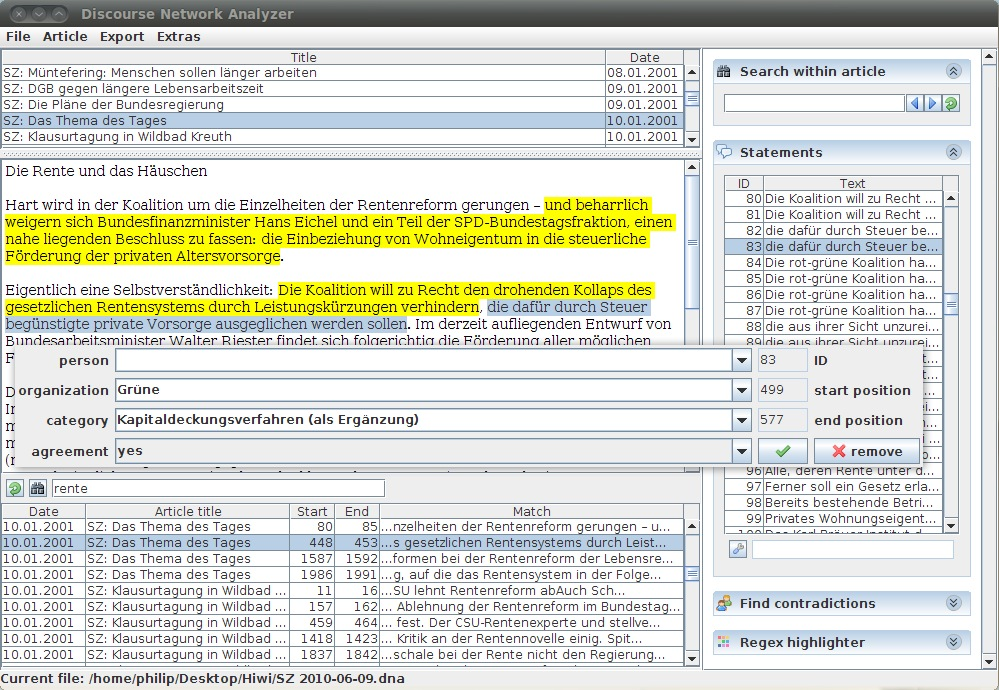
\includegraphics[scale=0.4]{dna-main.jpg}
\end{center}
\caption{The main window}
\label{main}
\end{figure}
Figure~\ref{main} shows the main window of \dnashort\ where newspaper articles, interviews, position papers, parliamentary protocols or other qualitative material can be inserted. Download the file \href{http://www.philipleifeld.de/cms/upload/Downloads/sample.dna}{\texttt{sample.dna}} from the \dnashort\ documentation section at \href{http://www.philipleifeld.de/discourse-network-analyzer-dna/documentation/}{\texttt{http://www.philipleifeld.de}}. This is a sample file with a couple of articles and statements. The articles are actually congressional hearings about the issue of climate change, taken from \citet{fisher2009understanding}.\footnote{The author wishes to thank Dana R. Fisher for contributing the sample data set. More information about the full data set and the political discourse on climate change in the U.S. is provided by \citet{fisher2009understanding}. A full-text archive of U.S. congressional hearings can be found at \url{http://www.gpoaccess.gov/chearings/}.} First, open the file by clicking on the 
\includegraphics[height=9px]{icons-open.png} \code{Open DNA file...} menu item.

\section*{Step 2: Navigating through articles}
\addcontentsline{toc}{section}{Step 2: Navigating through articles}
Once you have opened the file, you will see seven entries in the article table, ranging from January 26 to February 16, 2005. Each entry contains the speech of a business, NGO or government representative. The items in the article table are called ``articles'' (even though they were not taken from the news media in this case). If you click on an article, its corresponding text (i.\,e. the speech) will be displayed in the text area. Click on the entry ``109-1: Callahan, Kateri-NGO-Y'' now to see the speech of \emph{Kateri Callahan}, a representative of the \emph{Alliance to Save Energy}.

\section*{Step 3: Editing statements}
\addcontentsline{toc}{section}{Step 3: Editing statements}
Scroll down the text until you see a yellow text portion. This yellow text portion is called a ``statement''. A statement is a text portion where an actor reveals his/her opinion/belief/etc. about an issue. It depends on your theory what kind of information should be coded as statements. In the case of the sample file of \citet{fisher2009understanding}, different convictions about what should be done about climate change and how were coded as statements. Click on the yellow text starting with ``Energy Star\ldots'' now. A small window will pop up and reveal the details of the statement. The screenshot in figure~\ref{main} shows such a popup window roughly at the center of the screen. You will find four editable pieces of information:
\begin{itemize}
 \item the \emph{person} who makes the statement
 \item the \emph{organization} the speaker is affiliated with
 \item the \emph{category} which is raised by the actor (in this case the conviction that ``emmission legislation should regulate CO$_2$'')
 \item a dummy variable indicating whether the actor agrees with the category or not.
\end{itemize}
 It is possible to enter new information or select an actor/category from the combo boxes. The latter show all actor/category entries present in the current \dnashort\ file. \dnashort\ maintains lists of previous actors or categories on-the-fly, so it is not necessary to re-enter previously coded information. The advantage is an increase in reliability: It would lead to spurious results if typing errors prevented edges between actors or categories to be inferred from the text. Statements may be left incomplete if, for example, the person is not known. The ID field shows a unique identification number that every statement possesses, and which is not necessarily chronological. It cannot be changed by the user, but it can be used as a primary key if you want to record additional information about your statements in a separate database. If you click on the 
\includegraphics[height=9px]{icons-tick.png} button or somewhere outside of the popup window, all changes to the statement will be saved, and the statement popup window will be closed.

\section*{Step 4: Navigating through statements}
\addcontentsline{toc}{section}{Step 4: Navigating through statements}
The statement table in the sidebar on the right hand side shows all statements present in the current \dnashort\ file, together with their IDs. Click on an arbitrary statement. The corresponding article will be selected from the article table, the statement will be selected in the text window, and the statement popup window will be opened. Close the statement details again. If you click on the small wrench icon 
\includegraphics[height=9px]{bullet_wrench.png} underneath the statement table and then on \code{show statements in current article}, the list of statements will be filtered, and only those statements that occur within the currently selected article are shown. If you click on another article, this selection will change. It will always display the statements contained in the current article. The other filter options are based on regular expressions. Click the wrench icon 
\includegraphics[height=9px]{bullet_wrench.png} again, then \code{filter by category}, and enter the word ``economy'' into the text field right beside the button. Only statements with the category ``CO$_2$ legislation will not hurt the economy'' will be displayed. The statement filter works analogously for persons, organizations, statement IDs, and the text that is actually coded as a statement. The filters are based on regular expressions (see \url{http://www.regular-expressions.info} for details and instructions). For instance, if you type ``1[2-5]'' into the \code{statement ID} field, \dnashort\ will display all statements between 12 and 15.

\section*{Step 5: Creating statements}
\addcontentsline{toc}{section}{Step 5: Creating statements}
Click on the article of \emph{Christine Whitman} and select some words or lines of text with your mouse. Use your right mouse button to open the context menu. Now click on \code{
\includegraphics[height=9px]{icons-edit.png} Format as statement}. The highlighted text will become yellow. Congratulations, you have just created a statement. It should appear in the statement list on the right. If you have not added or removed a statement before, the ID of the statement should be ``37''. Click on the statement either in the text or in the statement list to open the statement popup window. Now you can enter the details of the statement or select them from the combo boxes. Since we have created this statement merely for the purpose of illustration, you can safely click on \code{
\includegraphics[height=9px]{icons-remove.png} remove} and confirm that you want to delete the statement from the file.
 
\section*{Step 6: Exporting co-occurrence networks}
\addcontentsline{toc}{section}{Step 6: Exporting co-occurrence networks}
\begin{figure}
 \centering
 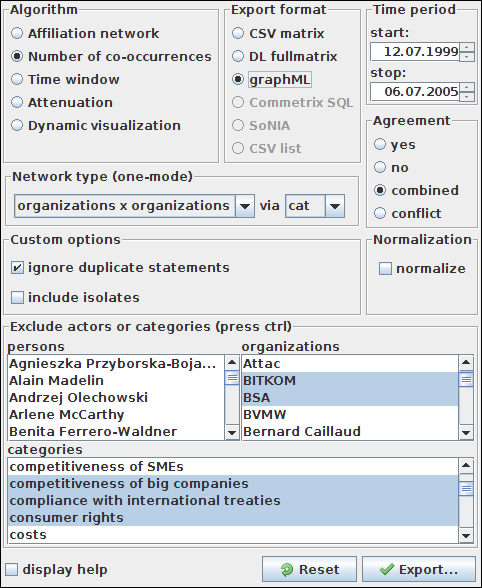
\includegraphics[scale=0.4]{dna-export.png}
\caption{Network export window}
\label{networkexport}
\end{figure}
Now you know the concept of a statement and how to deal with it in \dnashort. Next, we will export our structured data to a network file. This is the main purpose of the software. Click on the \code{
\includegraphics[height=9px]{icons-network.png} Network export...} entry in the \code{Export} menu. The network export window shown in figure~\ref{networkexport} will be opened. If you check the \code{display help} option, moving the mouse cursor over the various options of the network export window will show small tooltips with instructions. The default options will generate a network where two actors are connected by an edge if they share the same category. The more categories they share, the higher the edge weight will be. This is called a ``co-occurrence network'' or ``congruence network''.

For our example, select the category ``There should be legislation to regulate emissions'' in the category exclude list. The latter category is a very general one, with most actors agreeing on it. Hence it would not help us to examine the structure of the discourse network. By selecting it, statements with this category are ignored during the export procedure. Now click on \code{
\includegraphics[height=9px]{icons-tick.png} Export\ldots}, enter a file name, and click on \code{save}. This will produce a DL file, which can be read by \ucinet, \netdraw\footnote{\netdraw\ is delivered with \ucinet.}\ and \visonecolor. If you open the DL file in \netdraw, the network should look like the graph in figure~\ref{netdraw-cooc}. You can see two discourse coalitions of actors and one organization taking intermediate positions (i.\,e. agreeing on categories exhibited by both camps).
\begin{figure}
 \begin{center}
  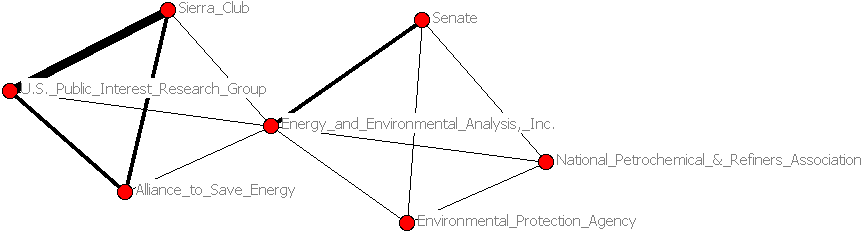
\includegraphics[scale=0.4]{netdraw.png}
 \end{center}
 \caption{Co-occurrence network of organizations}
 \label{netdraw-cooc}
\end{figure}
 
\section*{Step 7: Exporting affiliation networks}
\addcontentsline{toc}{section}{Step 7: Exporting affiliation networks}
If you want to understand why this structure looks the way it does, it is advisable to take a look at a (bipartite) affiliation network. While the co-occurrence network shows the relations between actors as a function of their agreement or disagreement with the same categories, an affiliation network shows directly how actors are connected to categories by positive (or negative) relations. To export an affiliation network, unselect the previously excluded category (press \code{Ctrl} on your keyboard while clicking on the entry), select \code{Affiliation network} in the \code{Algorithm} section, and select \code{yes} in the \code{Agreement} section. In this network, only positive relations (where agreement is coded as ``yes'') are included.\footnote{Combining positive and negative relations in the affiliation graph would return a multiplex network.} The resulting network DL file should look like figure~\ref{netdraw-affil}. You can now see that actors from both previously identified camps (the \emph{Environmental Protection Agency}, the \emph{Senate}, \emph{Sierra Club}, and the \emph{Alliance to Save Energy}) agree on having legislation to regulate emissions (this is why we excluded the category in the first place). Furthermore, you can see that \emph{Sierra Club} and the \emph{U.S. Public Interest Research Group} agree on four different categories. This explains the large edge weight in the co-occurrence graph, represented as the wide black line between the two organizations in figure~\ref{netdraw-cooc}. To get the full picture, you may want to look at the negative affiliation network (select \code{no} in the \code{Agreement} section) in order to be able to reconstruct the co-occurrence actor$\times$actor network.
\begin{figure}
 \begin{center}
  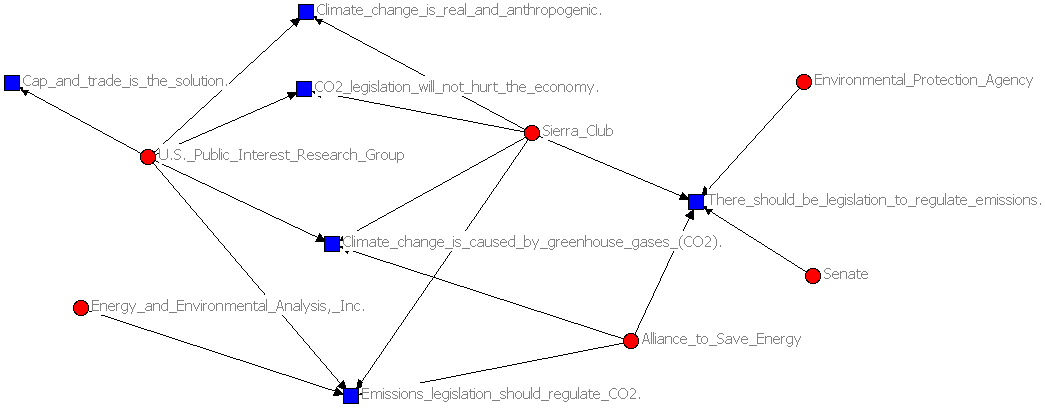
\includegraphics[scale=0.4]{netdraw-affil-yes.png}
 \end{center}
 \caption{Affiliation graph of positive agreement}
 \label{netdraw-affil}
\end{figure}

\section*{Step 8: Exporting statements to a CSV list}
\addcontentsline{toc}{section}{Step 8: Exporting statements to a CSV list}
Now imagine you would like to have a list of statements in Excel or a similar spreadsheet software. This can be useful to take stock of the overall picture or to combine the statements with other data for statistical purposes. Close the \code{Network export} window, go to the \code{Export} menu, select \code{List of statements}, and enter a file name. You can open the resulting CSV file in any spreadsheet software. It should look similar to the table depicted in figure~\ref{csvlist}.
\begin{figure}
 \begin{center}
  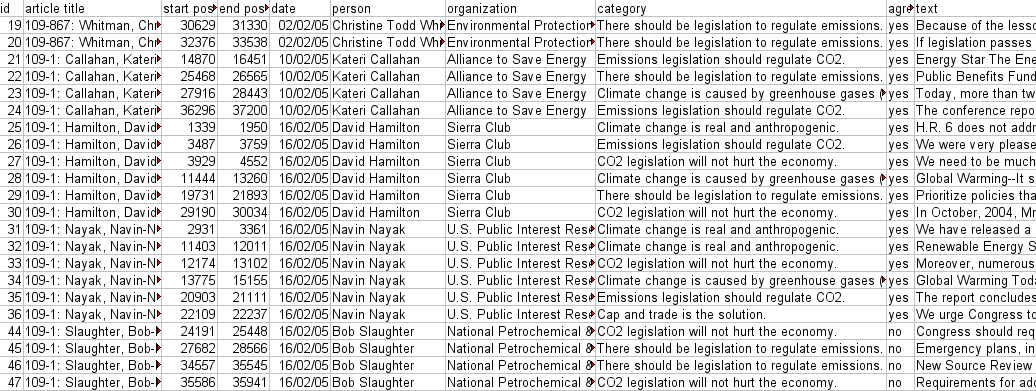
\includegraphics[scale=0.4]{csvlist.png}
 \end{center}
 \caption{CSV list of statements}
 \label{csvlist}
\end{figure}


\chapter{In-depth description}\label{indepth}
Figure~\ref{main} on page~\pageref{main} shows the main window where newspaper articles, interviews, position papers, parliamentary protocols or other qualitative material can be encoded. You first have to create an article entry by clicking on the \code{
\includegraphics[height=9px]{icons-newarticle.png} Add new article...} item in the \code{Article} menu and entering the relevant information (see section~\ref{article} for details). The menu also contains functions for opening, closing and saving \dnashort\ files (section~\ref{format}), deleting articles (section~\ref{article}), editing the title or date of an article (section~\ref{article}), recoding statements (section~\ref{recode}), exporting time series CSV files (section~\ref{statistics}) or network files (section~\ref{network}), and conducting a full-text search (section~\ref{search}).

\section{File format}\label{format}
\lstset{language=xml,
basicstyle=\ttfamily \color{black} \scriptsize,
keywordstyle=\color{darkblue},
identifierstyle=\color{gray},
commentstyle=\color{green!50!black!100},
stringstyle=\itshape \color{red},
breaklines=true,
breakatwhitespace=true,
numbers=left,
frame=single,
backgroundcolor=\color{blue!3},
caption={The \dnashort\ file format},
label={newformat}
}
\dnalong\ is based on an XML file format, which can be read and written by any text editor. Listing~\ref{newformat} shows the basic structure of a .dna file:

\begin{lstlisting}[breaklines=true,showstringspaces=false,frame=tlRB]
<?xml version="1.0" encoding="utf-8"?>
<discourse>
  <version>1.21</version>
  <metadata />
  <articles>
    <article>
      <text>put the article text here</text>
      <date>dd.mm.yyyy</date>
      <title>put the article title here</title>
      <statements>
        <statement>
          <id>numeric statement ID</id>
          <start>starting caret coordinate</start>
          <end>ending caret coordinate</end>
          <person>put the name of the person here</person>
          <organization>put organization here</organization>
          <category>put the category here</category>
          <agreement>yes</agreement>
        </statement>
        <!-- you can put more statements here -->
      </statements>
    </article>
    <!-- you can put more articles here -->
  </articles>
</discourse>
\end{lstlisting}

There may be a situation where you want to convert existing text data with actor and/or category tags into the \dnashort\ file format. Given the above XML file format specification, this is not particularly easy because statements are saved separately from the actual text, and caret coordinates are used to locate the beginning and end of a statement inside each article. In order to make life easier in this kind of situation, there is a second file format which can be read by \dnashort, but not written. This import file format stores statements directly inside the text. Listing~\ref{oldformat} shows the structure of the import file format.

\lstset{language=xml,
basicstyle=\ttfamily \color{black} \scriptsize,
keywordstyle=\color{darkblue},
identifierstyle=\color{gray},
commentstyle=\color{green!50!black!100},
stringstyle=\itshape \color{red},
breaklines=true,
breakatwhitespace=true,
numbers=left,
frame=single,
backgroundcolor=\color{blue!3},
caption={An alternative format specification for importing converted data},
label={oldformat}
}

\begin{lstlisting}[breaklines=true,showstringspaces=false,frame=tlRB]
<?xml version="1.0" encoding="utf-8"?>
<discourse>
  <article day="dd" month="mm" year="yy" title="title">
    put article text here <statement person="person" organization="organization" category="category" agreement="yes"> put statement text here </statement> put more article text here
    <!-- you can put more statements in the text -->
  </article>
  <!-- you can put more articles here -->
</discourse>
\end{lstlisting}

Please make sure your imported text is compatible with XML (e.\,g., it must not contain angle brackets and some other special characters; please look for the XML specification on the internet to obtain more information about incompatible characters and how to replace them by XML-compatible character sequences). Although the file format shown in listing~\ref{oldformat} is better for conversion, it has some disadvantages (e.\,g. non-overlapping statements). Therefore, the format shown in listing~\ref{newformat} is used to save files by default, and the format in listing~\ref{oldformat} is only used as an alternative input format.

The functions in the file menu can be used to open, save, save as, and close a .dna file, respectively.

\section{Dealing with articles}\label{article}
There are four things you can do with articles: import articles from another \dnashort\ file, add a new article to the current project file, edit the title or date of an article, and remove an article from the current project file.

\begin{figure}
	\centering
	\subfigure[Adding a new article\label{dna-newarticle}]{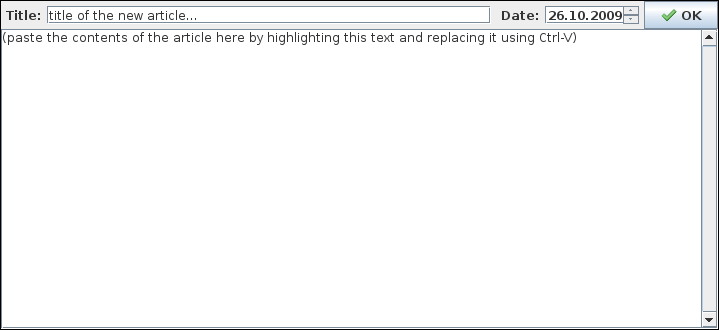
\includegraphics[scale=0.32]{dna-newarticle.png}}\\
	\subfigure[Importing articles\label{dna-import}]{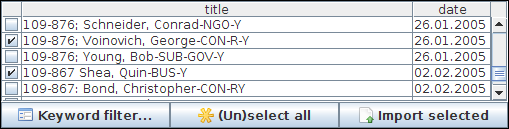
\includegraphics[scale=0.32]{dna-import.png}}
	\hspace{1cm}
	\subfigure[Edit title/date\label{dna-changetitle}]{
\includegraphics[scale=0.32]{dna-changetitle.png}}
	\caption{Operations on articles}
	\label{article-screenshots}
\end{figure}

The \code{
\includegraphics[height=9px]{icons-newarticle.png} Add new article...} menu item opens a new window upon mouse click, where you can enter the title, date and text of a new article. Figure~\ref{dna-newarticle} shows a screenshot of this window. Please make sure you enter the date correctly because otherwise the algorithms for longitudinal data (described in section~\ref{algorithm}) will not work properly. The title may include any kind of information, for instance a unique ID if you plan to collect additional information about the articles in a separate database. Duplicate article titles are not allowed. You can copy your article from a website or any other text source and paste it in the text field. Single line breaks are automatically removed, while double line breaks (paragraph breaks) are preserved. Some escape sequences and special characters are automatically removed when text is inserted. The \code{
\includegraphics[height=9px]{icons-deletearticle.png} Delete selected article} function will completely remove an article from the \dnashort\ file, including its statements.

If there is more than one person working on the same project at the same time, it is usually difficult to merge the files manually later on. To avoid trouble with duplicate statement IDs and article names, the function \code{import articles} (
\includegraphics[height=9px]{icons-import.png}) can be used. A screenshot is shown in figure~\ref{dna-import}. You can select the articles from a .dna file that you would like to insert into your current document, and \dnashort\ will take care of duplicates, etc. You can also automatically select or unselect all articles by pressing the button in the middle. The left button allows to select articles by keyword filter, i.\,e., you enter a regular expression (such as \code{\^{}NYT:}), and \dnashort\ will select all articles starting with \code{NYT:}. Section~\ref{regex} provides more details on regular expressions.

There is also a function in the article menu to \code{edit} the title or date of the currently selected article (\code{
\includegraphics[height=9px]{icons-editarticle.png} Rename selected article...}). This will open the window shown in figure~\ref{dna-changetitle}. Again, duplicate titles are not permitted.

\section{Recoding statements}\label{recode}
The item \code{
\includegraphics[height=9px]{icons-recode.png} Recode statements...} in the \code{Extras} menu opens a recoding function for statements. A screenshot is presented in figure~\ref{dna-recode}. In the upper part of the window, you can select the statements you want to recode based on the \code{person}, \code{organization} and \code{category} fields. The recode operations specified in the lower part of the window will be applied to all statements matching the selection. If several criteria are selected, the intersection (e.\,g. all statements with a certain actor \emph{and} and a certain category) is selected, not the union (an \emph{or} operator). There are two possible operations: removing all matching statements completely, and recoding them. The recoding operation makes use of wildcards (\code{\%o} stands for the organization, \code{\%p} for the person and \code{\%c} for the category). It is possible to enter any kind of text in any of the three fields; for example entering ``Environmental Protection Agency'' into the \code{organization} field will simply rename the organization of all matching statements. In addition to this simple renaming, wildcards can be combined with normal text (e.\,g. \code{\%o (NGO)} will add a suffix to the \code{organization} field). This is particularly useful if some organizational actors should be coded as individuals (e.\,g. \code{\%p (\%o)}).
\begin{figure}
 \centering
 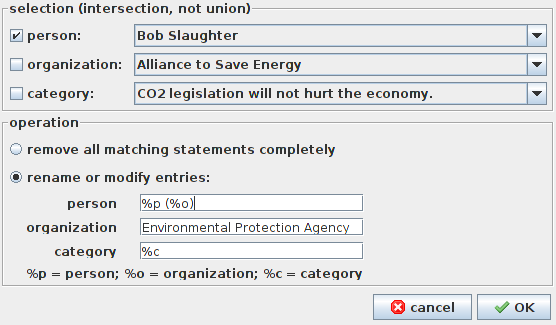
\includegraphics[scale=0.4]{dna-recode.png}
 \caption{Recoding window}
 \label{dna-recode}
\end{figure}

\section{Regular expressions highlighter}\label{regex}
The sidebar on the right contains a regular expressions manager. In this panel, you can specify keywords which are highlighted in the text, along with a text color. These keywords are in fact regular expressions, an extremely powerful tool to match actors, categories or any kind of text.\footnote{The websites \url{http://www.regular-expressions.info} and \url{http://java.sun.com/j2se/1.4.2/docs/api/java/util/regex/Pattern.html} provide details on how to use regular expressions.} The regex function implemented in \dnashort\ relies on case-insensitive expressions. The keywords are automatically saved in the  \code{.dna} file. The purpose of the regex highlight function is to assist the user in the encoding of statements by rendering the coding procedure semi-automatic. Coding is much faster if a proper list of keywords is specified in advance, so actors and categories can easily be found when eyeballing the document. Here are some examples:
\begin{description}
 \item[\textasciicircum EPA\textdollar] will find the word ``EPA'' only if it is not part of another word, i.\,e. ``Nepal'' is not found.
 \item[(G.W.)$|$(G. W.)$|$(George W.)$|$(George)$|$(George W) Bush] will find several name va\-ri\-a\-tions.
 \item[CO[0-9{]}] will find ``CO2'', but also ``CO3'', ``CO4'', etc.
\end{description}

\section{Within-actor contradictions}
The sidebar on the the right contains a function which searches for self-contradictions of actors (\code{
\includegraphics[height=9px]{icons-group.png} Find contradictions}). The results are displayed in a tree view. The tree contains direct contradictions within persons. For example, if a politician uses a category in a positive way in one article and uses the same category in a negative way somewhere else, this is counted as a within-person contradiction. The tree lists all contradictions in the file in a hierarchical way. Figure~\ref{dna-contradictions} shows a screenshot.

\begin{figure}
 \begin{center}
  \subfigure[\label{dna-contradictions}]{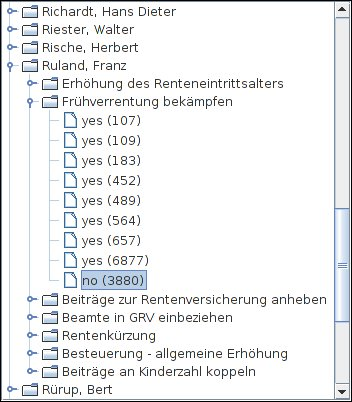
\includegraphics[scale=0.4]{dna-contradictions.jpg}} \hspace{0.5cm}
  \subfigure[\label{dna-statistics}]{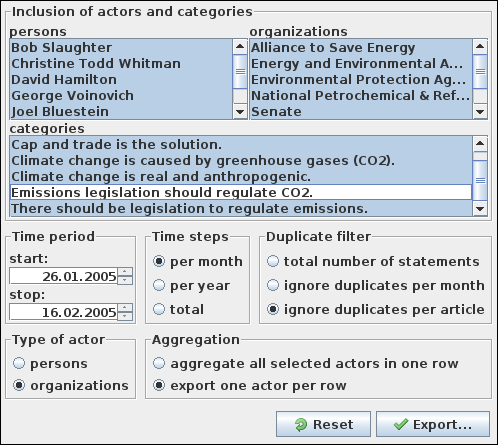
\includegraphics[scale=0.4]{dna-statistics.png}}
 \end{center}
 \caption{Within-actor contradictions and the statistics export component}
 \label{dna-contradictions-statistics}
\end{figure}

If you click on a statement in the tree, \dnashort\ will highlight the statement in the main window. You can thus use the contradiction report as a navigation instrument. It basically serves to identify either coding inconsistencies or learning behavior of actors over time. You can choose if you want to examine self-contradictions of persons or of organizations.

\section{The bottom bar}
The item \code{Toggle bottom bar (show/hide)} in the \code{Extras} menu shows or hides a panel with additional functions: a full-text search function and an attribute manager for actors. The items in the \code{Extras} menu can be used to specify which function should be shown in the bottom bar.

\subsection{Full-text search}\label{search}
This is a search panel as shown at the bottom of figure~\ref{main} on page~\pageref{main}. You can enter a regular expression and search for it in the whole file across articles. A table will display the results. If you click on a result, the corresponding article will be opened, and the matched text will be highlighted.

\subsection{Organizations}
\begin{figure}
 \centering
 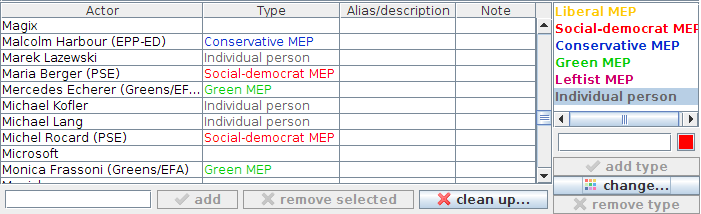
\includegraphics[scale=0.4]{dna-attributes.png}
 \caption{Actor attributes}
 \label{dna-attributes}
\end{figure}
If you activate \code{Show organizations in bottom bar}, there will be a panel where you can enter additional information about the organizations in the data set (see figure~\ref{dna-attributes}). There is a field for the \code{type} of organization, where you can select the actor group this organization belongs to. You can specify the types using the list on the right. A color is associated with each type, and you can change the name or the color of the type at any time in the whole data set. You may, for example, specify the tag ``socialist interest group'' with a red color and assign this tag to all organizations which have socialist goals. The second field, \code{alias/description} is reserved for an alternative name of the organization. If you use abbreviations as organization names, it may be helpful to enter the full names of the organizations in the alias field. If you don't use abbreviations, it may be helpful to add a description. The note field can contain arbitrary kinds of text. Currently, the attribute data are used in three ways:
\begin{enumerate}
 \item You can export the table of attributes to a CSV file from the \code{Export} menu.
 \item When you open a statement popup window, the organizations in the combo box will be colored according to the selected organization type. You can switch off this behavior in the \code{Extras} menu by deactivating the option \code{Use colors for actor selection}.
 \item The attribute data are included in the network export when you use graphML files (e.\,g., for \visone). This makes it easier to visualize the network. Additionally, the vertex color uses the color of the type tag.
\end{enumerate}
However, other network formats currently do not make use of the attribute data. Support for attribute data in other network export formats may be added in future versions.

You can also add new organizations to the list. As long as an organization is not contained in any statement, it will be highlighted with a red background color. You can delete all of these organizations from the list if you click on \code{clean up...} or only the selected red organizations by clicking on \code{remove selected}. Organizations which are currently used somewhere in a statement cannot be removed.

\subsection{Persons}
This is the same as the organizations panel, but for persons.


\section{Exporting time series statistics}\label{statistics}
The menu item \code{Time series statistics...} in the \code{Export} menu starts the statistics export component shown in figure~\ref{dna-statistics}. The purpose is the extraction of time-series information about statement frequencies. The output will be a table with actors as the rows and time periods as the columns. The cells contain the number of statements of each actor per time period. The resulting CSV file can be read by \excel, \calc\ or any other spreadsheet software. There are six option panes in the statistics component:

\subsection{Inclusion of actors and categories}
The upper three lists show all persons, organizations and categories in the .dna file. By default, all entries are selected. You can select or deselect entries with your mouse while pressing the \code{Ctrl} key on your keyboard. If an entry is not selected, all statements containing this entry will be ignored by the statistics export procedure.

\subsection{Time period}
Statements are only included in the statistics export if they are within the range of dates. By default, the first date and the last date present in the .dna file will be used.

\subsection{Time steps}
This option governs whether the statement frequencies will be aggregated into one number per actor (\code{total}), whether they will be aggregated by \code{month} (i.\,e., the number of statements of each actor will be exported for each month separately), or whether they will be aggregated by \code{year} (counts how many statements each actor has made in each year).

\subsection{Duplicate filter}
The option \code{total number of statements} simply counts how many statements an actor has made overall in each time period. This implies that repeated statements are counted several times. The option \code{ignore duplicates per month}, in contrast, will count repeated statements only once per month. As soon as a new calendar month has started, previously excluded statements a counted again, but not more than once per month and per actor. \code{Ignore duplicates per year} is the same as before, but this time on an annual basis.

\subsection{Type of actor}
If you select \code{organizations}, this will aggregate the frequencies organization-wise, while the \code{person} option will aggregate frequencies per person, no matter what organization the person is affiliated with.

\subsection{Aggregation}
By default, frequencies are aggregated for each actor separately. If you want to obtain a simple time series that does not distinguish between actors (i.\,e., an overall frequency assessment), you should select the option \code{aggregate all selected actors in one row} for convenience.

\section{Exporting network data}\label{network}
Clicking on the network export button will convert your qualitative codes into networks. Figure~\ref{networkexport} reveals the currently implemented export options. They work as follows:

\subsection{Algorithm}\label{algorithm}
There are currently six different algorithms for network generation.

\subsubsection{Affiliation network}
This creates a bipartite network, e.\,g. organizations$\times$catego\-ries or per\-sons$\times$or\-ga\-ni\-za\-tions. An edge is created between a class 1 vertex and a class 2 vertex if there is a statement that contains both of them.

The affiliation algorithm has two options: The \code{include isolates} option will also include all actors (or categories) that do not have any links to categories (or actors). This may be useful, for instance, if you export several time slices or several relations separately and want to combine the different matrices later on.

The other option is to \code{ignore duplicates}. If \code{yes} or \code{no} is set in the \code{agreement} option panel (described in section~\ref{agreement}) and if \code{ignore duplicates} is activated, the resulting network will be binary, i.\,e. an actor either refers to a category at least once, or (s)he does not refer to the category. This is reflected by the presence or absence of a tie. If \code{yes} or \code{no} is set and the \code{ignore duplicates} option is unchecked, the resulting network will contain weighted edges, and the edge weight reflects the number of times the actor cites the category in a positive or negative way (depending on the \code{agreement} option).

If \code{combined} is set in the \code{agreement} option panel, both positive and negative citations of categories will be counted. However, the behavior deviates from the other algorithm in the following respect: If the \code{ignore duplicates} options is enabled, the resulting network will be multiplex, i.\,e. an edge value of 0 represents no connection, a value of 1 indicates that the actor only agrees with the category, a value of 2 reflects only disagreement with the category, and a value of 3 indicates that the actor both agrees and disagrees with the category. These information can be used in \visone\ or \netdraw\ to apply different colors or line types to the edges. If the \code{ignore duplicates} option is disabled, positive citations will be added to the edge weight and negative ones will be subtracted. For example, if an actor agrees five times with a category and disagrees seven times with the same category, the edge weight will be -2. Values above 0 indicate overall agreement while negative values indicate overall disagreement.

Unchecking the \code{ignore duplicates} or the \code{include isolates} option has no effect when exporting to a CSV list file. This is a simple nodelist format which merely lists the affiliations of a vertex per line. The format can be used to get an overview of different organizational affiliations of individual persons, or vice-versa.

Affiliation networks can also be exported to \sonia\ for dynamic network visualization. The result will be a two-mode .son file. Please refer to the subsection on dynamic visualization for more details.

\subsubsection{Number of co-occurrences}
This creates an adjacency network, e.\,g. organiza\-tions$\times$organizations or ca\-te\-go\-ries$\times$ca\-te\-go\-ries. An edge is created e.\,g. between two organizations if they share a category, or between two categories if they share an actor. The edge weight reflects the number of common items. If, for example, organization 1 refers to three concepts which organization 2 also refers to, an edge with a weight of 3 is created between organization 1 and organization 2. The same is possible for persons or for categories.

There are two options for this algorithm: If you check \code{include isolates}, actors without any overlap with other actors are included in the network file. This is helpful if you export several time slices and want to combine the files later on. If isolates are not included, it may become difficult to match the matrices because they differ in their lengths. This may also be the case if you export single relations and plan to join them in a multiplex network. The other option, \code{ignore duplicate statements}, guarantees that edge weights are not overestimated simply because an actor repeats the same statement several times. Edges are essentially \emph{binary per relation}, i.\,e. if two actors share five different categories three times each, the edge weight will be five, no matter how often the statements are repeated. But if you uncheck the option \code{ignore duplicate statements}, frequencies are counted, and the edge weight in the above example will be 45 because $3 \cdot 3 \cdot 5 = 45$.
 
Although the above examples are based on actors, it is as well possible to compute a co-occurrence network of categories, where two categories have an edge weight of $w$ if they are both used by $w$ different actors. Similarly, you can generate an interlocking-directorates network of persons$\times$persons via common organizational memberships.

\subsubsection{Time window}
\begin{figure}
  \centering
  \begin{tikzpicture}
  
    \draw[line width=1pt] (2cm,0cm) -- (9cm,0cm)
      node [below=0.1cm] at (5.5cm,0.1cm) {$\bar{d} = d^e - d^b$};
    \draw[line width=1pt] (2cm,-0.1cm) -- (2cm,0.1cm) node [below=0.1cm] {$d^b$};
    \draw[line width=1pt] (9cm,-0.1cm) -- (9cm,0.1cm) node [below=0.1cm] {$d^e$};
    \draw[dashed, line width=1pt] (1cm,0cm) -- (2cm,0cm);
    \draw[dashed, line width=1pt] (9cm,0cm) -- (10cm,0cm);
  
    \draw[line width=1pt, color = red] (0cm,1cm) -- (2cm,1cm)
      node [below=0.1cm] at (1cm,1.1cm) {$\bar{w}$}
      node [color = black, left = 0.2cm] at (0cm,1cm) {$t=0$};
    \draw[line width=1pt, color = red] (0cm,0.9cm) -- (0cm,1.1cm) node [below=0.1cm] {$w^b$};
    \draw[line width=1pt, color = red] (2cm,0.9cm) -- (2cm,1.1cm) node [below=0.1cm] {$w^e$};
  
    \draw[line width=1pt, color = red] (1cm,2cm) -- (3cm,2cm)
      node [color = black, left = 0.2cm] at (0cm,2cm) {$t=1$};
    \draw[line width=1pt, color = red] (1cm,1.9cm) -- (1cm,2.1cm) node [below=0.1cm] {$w^b + s$};
    \draw[line width=1pt, color = red] (3cm,1.9cm) -- (3cm,2.1cm) node [below=0.1cm] {$w^e + s$};
  
    \draw[line width=1pt, color = red] (2cm,3cm) -- (4cm,3cm)
      node [above] at (3cm,3.1cm) {$\bar{w}$}
      node [color = black, left = 0.2cm] at (0cm,3cm) {$t=2$};
    \draw[line width=1pt, color = red] (2cm,2.9cm) -- (2cm,3.1cm) node [below=0.1cm] {$w^b + 2s$};
    \draw[line width=1pt, color = red] (4cm,2.9cm) -- (4cm,3.1cm) node [below=0.1cm] {$w^e + 2s$};
  
    \draw[line width=1pt, color = red] (9cm,4cm) -- (11cm,4cm)
      node [color = black, left = 0.2cm] at (0cm,4cm) {$t=n$};
    \draw[line width=1pt, color = red] (9cm,3.9cm) -- (9cm,4.1cm) node [below=0.1cm] {$d^e = w^b + ns$};
    \draw[line width=1pt, color = red] (11cm,3.9cm) -- (11cm,4.1cm) node [above] {$d^e + \bar{w} = w^e + ns$};
  
    \draw[line width=1pt, color = blue] (3cm,1cm) -- (4cm,1cm)
      node [below=0.1cm] at (3.5cm,1cm) {$s$};
    \draw[line width=1pt, color = blue] (3cm,1cm) -- (3cm,1.1cm);
    \draw[line width=1pt, color = blue] (4cm,1cm) -- (4cm,1.1cm);
  
  \end{tikzpicture}
  \caption{The time window algorithm}
  \label{timewindow}
\end{figure}
 
Statements are context-sensitive. If an actor refers to a category in 1995 and again in 2005, the meaning of the category in the discourse may have changed in the meantime. This leads to an overestimation of edges between actors and eventually to a higher density of the measured network. The time window algorithm offers a solution: It runs a time window of a specified size (the number of days is called the chaining parameter) chronologically through the discourse from the beginning to the end. Whenever two actors make a statement within the time window, an edge is created. If the edge has already been present, the edge weight is increased. If at least one of the statements is made outside of the time window, the link is not established. This guarantees context sensitivity of the resulting network. The drawback is that edge weights may become quite large, so you may consider to normalize or dichotomize the data. A second parameter, the shift parameter, governs the number of days by which the time window is moved at every step. If you prefer discrete, non-overlapping time units, you may set the shift parameter to the size of the chaining parameter (i.\,e. its maximum value). If you prefer a more precise continuous-time result, you may set the parameter to 1. Figure~\ref{timewindow} illustrates how the time window is moved through the discourse.

\subsubsection{Attenuation}
It may be interesting to add another assumption to the model: If actor 1 makes a statement, and a couple of days later, actor 2 makes the same statement, actor 2 is likely to refer to actor 1 by making this statement. It is thus possible to create a directed adjacency graph of referrals. The edge weight between actor 2 and actor 1 is proportional to the probability that actor 2 is really referring to actor 1. Now the trick is to infer this probability from the actual empirical data by using the time that has passed since the statement of actor 1. If, for example, actor 2 makes the same statement immediately on the next day, (s)he is very likely to refer to actor 1, so the edge weight should be large. If, in contrast, actor 2 makes the same statement two years later, (s)he is not very likely to refer to actor 1, so the edge weight should be small. The probability of referral is assumed to be declining exponentially with time, i.\,e., a statement which is made after five days is added to the edge weight as $e^{-\lambda \cdot 5}$, etc. The decay constant $\lambda$ can be set arbitrarily. A value of $0.1$ should work in many cases because it assigns a value greater than 0.5 to statements made within about one week after the initial statement. The exponentially transformed time is added to the existing edge weight, for all pairs of actors over all statements. This produces a very detailed network of referrals. However, you should be aware of the additional assumptions this kind of network is based upon. Figure~\ref{atten} provides an illustration for the two-player case.

\begin{figure}
\centering
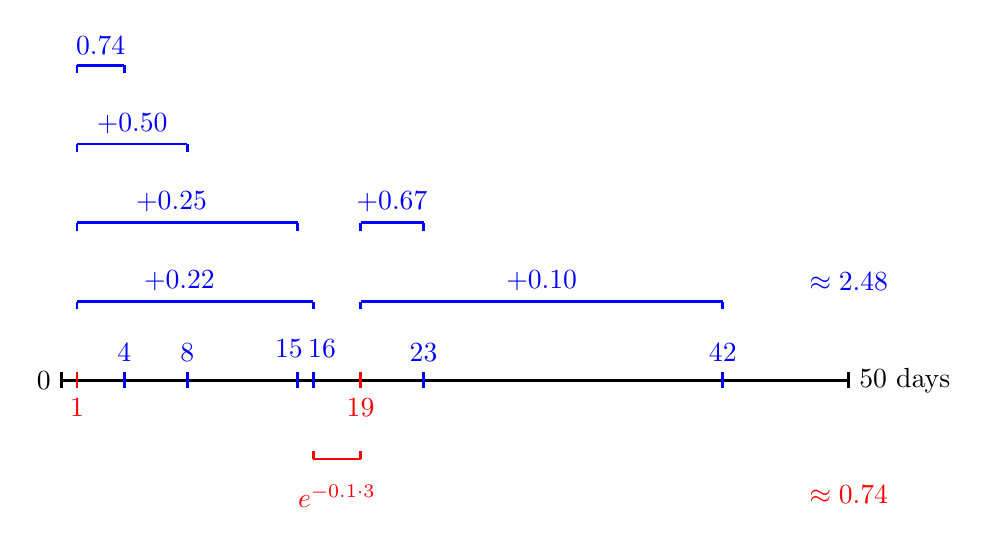
\begin{tikzpicture}

  \draw[line width=1pt] (0cm,0cm) -- (10cm,0cm)
    node [right] {50 days}
    node [left] at (0cm,0cm) {0};
  \draw[line width=1pt] (0cm,-0.1cm) -- (0cm,0.1cm);
  \draw[line width=1pt] (10cm,-0.1cm) -- (10cm,0.1cm);
  \draw[line width=1pt, color=red] (0.2cm,-0.1cm) -- (0.2cm,0.1cm)
    node [color = red, below=0.2cm] {$1$};
  \draw[line width=1pt, color=red] (3.8cm,-0.1cm) -- (3.8cm,0.1cm)
    node [color = red, below=0.2cm] {$19$};
  \draw[line width=1pt, color=blue] (0.8cm,-0.1cm) -- (0.8cm,0.1cm)
    node [color = blue, above] {$4$};
  \draw[line width=1pt, color=blue] (1.6cm,-0.1cm) -- (1.6cm,0.1cm)
    node [color = blue, above] {$8$};
  \draw[line width=1pt, color=blue] (3cm,-0.1cm) -- (3cm,0.1cm)
    node [color = blue, above=0.3cm, left=-0.2cm] {$15$};
  \draw[line width=1pt, color=blue] (3.2cm,-0.1cm) -- (3.2cm,0.1cm)
    node [color = blue, above=0.3cm, right=-0.2cm] {$16$};
  \draw[line width=1pt, color=blue] (4.6cm,-0.1cm) -- (4.6cm,0.1cm)
    node [color = blue, above] {$23$};
  \draw[line width=1pt, color=blue] (8.4cm,-0.1cm) -- (8.4cm,0.1cm)
    node [color = blue, above] {$42$};

  \draw[line width=1pt,color=blue] (0.2cm, 4cm) -- (0.8cm,4cm)
    node [color = blue, above] at (0.5cm,4cm) {$0.74$};
  \draw[line width=1pt,color=blue] (0.2cm, 3.9cm) -- (0.2cm,4cm);
  \draw[line width=1pt,color=blue] (0.8cm, 3.9cm) -- (0.8cm,4cm);

  \draw[line width=1pt,color=blue] (0.2cm, 3cm) -- (1.6cm,3cm)
    node [color = blue, above] at (0.9cm,3cm) {$+ 0.50$};
  \draw[line width=1pt,color=blue] (0.2cm, 2.9cm) -- (0.2cm,3cm);
  \draw[line width=1pt,color=blue] (1.6cm, 2.9cm) -- (1.6cm,3cm);

  \draw[line width=1pt,color=blue] (0.2cm, 2cm) -- (3cm,2cm)
    node [color = blue, above] at (1.4cm,2cm) {$+ 0.25$};
  \draw[line width=1pt,color=blue] (0.2cm, 1.9cm) -- (0.2cm,2cm);
  \draw[line width=1pt,color=blue] (3cm, 1.9cm) -- (3cm,2cm);

  \draw[line width=1pt,color=blue] (0.2cm, 1cm) -- (3.2cm,1cm)
    node [color = blue, above] at (1.5cm,1cm) {$+ 0.22$};
  \draw[line width=1pt,color=blue] (0.2cm, 0.9cm) -- (0.2cm,1cm);
  \draw[line width=1pt,color=blue] (3.2cm, 0.9cm) -- (3.2cm,1cm);

  \draw[line width=1pt,color=blue] (3.8cm, 2cm) -- (4.6cm,2cm)
    node [color = blue, above] at (4.2cm,2cm) {$+ 0.67$};
  \draw[line width=1pt,color=blue] (3.8cm, 1.9cm) -- (3.8cm,2cm);
  \draw[line width=1pt,color=blue] (4.6cm, 1.9cm) -- (4.6cm,2cm);

  \draw[line width=1pt,color=blue] (3.8cm, 1cm) -- (8.4cm,1cm)
    node [color = blue, above] at (6.1cm,1cm) {$+ 0.10$}
    node [color = blue, above] at (10cm,1cm) {$\approx 2.48$};
  \draw[line width=1pt,color=blue] (3.8cm, 0.9cm) -- (3.8cm,1cm);
  \draw[line width=1pt,color=blue] (8.4cm, 0.9cm) -- (8.4cm,1cm);

  \draw[line width=1pt,color=red] (3.2cm, -1cm) -- (3.8cm,-1cm)
    node [color = red, below=0.2cm] at (3.5cm,-1cm) {$e^{-0.1 \cdot 3}$}
    node [color = red, below=0.2cm] at (10cm,-1cm) {$\approx 0.74$};
  \draw[line width=1pt,color=red] (3.2cm, -0.9cm) -- (3.2cm,-1cm);
  \draw[line width=1pt,color=red] (3.8cm, -0.9cm) -- (3.8cm,-1cm);

\end{tikzpicture}
\caption{An example of partial edge weights in the attenuation algorithm}
\label{atten}
\end{figure}

\subsubsection{Dynamic visualization}
This algorithm generates a list of edges, where each edge is affiliated with a date. If, say, organization 1 makes a statement on the 1\textsuperscript{st} of July, and organization 2 makes the same statement on the 23\textsuperscript{rd} of August, an edge between 1 and 2 is created, and the creation date is the 23\textsuperscript{rd} of August. Once having produced such an edgelist, the network can be visualized in a dynamic, continuous-time way by employing the tool \commetrix\ (\url{http://www.commetrix.de}). The advantage is that you can now directly observe how the network evolves over time and on what dates interesting changes happen. \commetrix\ also offers a time window visualization where older edges are faded out. Please look at the description of the \commetrix\ file format below in order to understand how you can use it in your project. \par For \commetrix, there are two parameters: A \code{backward window} determines, from the perspective of the second statement, how many days to go back in time in order to create edges. In the above example, a backward window of 20 days would not establish an edge between the actor on the 1\textsuperscript{st} of July and the other actor on the 23\textsuperscript{rd} of August, but a backward window of 60 days would. The other parameter is the (arbitrary) \code{network name} to be used in the \commetrix\ file. \par An alternative dynamic visualization software is \sonia\ (\url{http://www.stanford.edu/group/sonia/}). \sonia\ is free to use, but \commetrix\ seems to offer much better visualization capabilities for the type of data produced by the \dnalong.  If you use the \sonia\ file format, there is an additional parameter, the \code{forward window}. It determines how long an edge is valid before fading out in the dynamic visualization.

\subsubsection{List of statements}
This exports a plain list of statements without any network information as a CSV file. Columns include the date of a statement, the person, organization, category, agreement and the contents (i.\,e. the text that was encoded).


\subsection{Export format}

\subsubsection{CSV matrix}
A comma-separated value text file with semicolons as column separators. The file will contain a socio-matrix with the complete network and the labels. CSV files can be opened in any text editor or spreadsheet software like \excel\ or \calc.

\subsubsection{DL fullmatrix}
A text format for networks. The fullmatrix specification means that the file will contain a socio-matrix with the complete network and the labels. DL files can be imported by the network-analytic software \ucinet\ (\url{http://www.analytictech.com}) and then exported into a variety of formats from \ucinet. DL fullmatrix files can also be opened by the visualization software \visonecolor\ (\url{http://www.visone.info}). In some cases, however, \visonecolor\ does not display the labels properly. In these cases, importing and re-exporting the DL file in \ucinet\ will do the trick.

\subsubsection{graphML}
The graphML file format is based on XML and is the native format of \visonecolor\ (\url{http://www.visone.info}). The specification of the format can be found at \url{http://graphml.graphdrawing.org}. Please note that coordinates of the vertices will not be exported, i.\,e. all nodes will at first appear at the same location. You should use layout algorithms to assign X--Y coordinates to the vertices.

\subsubsection{Commetrix SQL}\label{cmx}
This is a text file format that contains data generated by the \code{edgelist with time stamp} algorithm (see above). Here is how to use it: The result of the export will be a .sql file. You should send this file to the developers of \commetrix\ (\url{http://www.commetrix.de}). They will -- for a small fee -- convert the .sql file to a .CMX file and send it back to you. You can use this .CMX file in the CMX Analyzer to visualize your data. Alternatively, you can purchase a license for a tool called CMX Producer from the \commetrix\ developers and create your own CMX files out of the .sql files. This is a little bit more expensive but you may create an unlimited number of CMX files. Please obtain CMX Analyzer and information about the rates and licenses from the \commetrix\ team. Academic or private rates are not very expensive.

\subsubsection{SoNIA}
This format is similar to the \commetrix\ format and can be used with the dynamic visualization software \sonia. A disadvantage compared to \commetrix\ is that relative durations are saved instead of absolute time stamps.

\subsubsection{CSV list}
A comma-separated value text file which can be used for the statement list algorithm. Semicolons are used as column separators. CSV files can be opened in any text editor or spreadsheet software like \excel\ or \calc.


\subsection{Time period}
Only statements between the start date and the stop date will be considered for export. The default values are the first and the last date found in the .dna file.

\subsection{Normalization}
Edge weights between actors are usually affected by the propensity of an actor to make a statement. For example, a government agency concerned with the labor market is more likely to make a statement about the pension system than an interest group concerned with gender equality. This difference is partly due to institutional roles. As a consequence, some actors will occupy central positions in the discourse network just because they are more mediagenic or because of their institutional role. If you want edge weights to be independent of this, you should use edge weight normalization. There are three different edge weight transformations, depending on the algorithm that you use:

\begin{description}
 \item[Co-occurrence normalization:] Divide the edge weight by the average number of distinct categories used by both actors involved in an edge.
 \item[Time window normalization:] This works like the co-occurrence normalization, but on top of that, it divides the resulting value by the number of time steps taken by the time window, and multiply it by a constant called $\alpha$ in order to get an appropriate scale. $\alpha$ can be set in the custom options panel of the time window algorithm. Its default value is 100.
 \item[Attenuation normalization:] This is the most complicated normalization algorithm. Normalization is already carried out during edge weight calculation. Imagine a situation where actor 1 makes a statement on day 0, and actor 2 repeats the same statement on days 4, 10 and 15. According to the attenuation algorithm, the edge from actor 2 to actor 1 should have a weight of $e^{-\lambda \cdot 4} + e^{-\lambda \cdot 10} + e^{-\lambda \cdot 15} = 1.26$ if $\lambda = 0.1$. The normalization option now divides this value by the number of equal statements that actor 2 makes, before adding up the values across statements and actors. We would thus add a value of $\frac{1.26}{3} = 0.42$, which corresponds to the \emph{average} attenuated duration between actor 2 and actor 1 for this specific statement. The resulting values are added up for each statement that is shared by the two actors.
\end{description}
Please be aware that the normalization algorithms are in an experimental stage, so they may produce biased results.

\subsection{Agreement}\label{agreement}
If you select \code{yes}, only statements where agreement was encoded as ``yes'' are considered in the export process. If you select \code{no}, only statements where agreement was encoded as ``no'' are considered in the export process. \code{Combined} will produce adjacency networks where actor 1 and actor 2 both agree or both disagree. In the case of the affiliation algorithm, the bipartite graph will contain agreement as well as disagreement relations without making a distinction. The \code{conflict} option will yield a network where actor 1 agrees and actor 2 disagrees or vice-versa. This is useful for analyzing direct contradictions between actors.

\subsection{Exclude lists}
There are three lists showing all the persons, organizations and categories from the .dna file. You can select items that you want to exclude from the export process. If you do this, all statements that contain excluded items will be skipped during export. To (un)select multiple entries from a list, you can press \code{Ctrl} while (un)selecting additional items.

\chapter{rDNA. A Package to Control Discourse Network Analyzer from R}
rDNA is an R package that allows to integrate the \dnalong\ into the statistical programming environment R.

\section{Motivation}
R is becoming increasingly popular as a platform for social network analysis (see, for example, the \href{http://www.statnetproject.org}{statnet project}). The focus of DNA is the extraction of network data from manually encoded textual discourses. Bringing together the data-generating software and the methods for processing these data therefore seems quite natural.

Before the development of rDNA, the easiest way to get \dnashort\ data into R was to export a network to a CSV file and then import this CSV file in R using the \code{read.table()} command. This can quickly become tedious because every time even minor parts of the analysis are changed, the data have to be re-exported from \dnashort\ and re-imported into R. With rDNA, in contrast, the analyst can directly pull the desired network data from a .dna file without going through the whole user interface and export options of \dnashort. Or, if desired, rDNA allows to start the coding window of \dnashort from within R in order to provide an interactive content analysis solution for R (similar to the \href{http://rqda.r-forge.r-project.org}{RQDA project}, but with an additional focus on network analysis).

Installation instructions are provided online.

\section{Functionality}
As of version 1.2, rDNA provides seven R functions:
\begin{description}
 \item[dna.init] initializes the connection between R and \dnashort.
 \item[dna.gui] starts the user interface of \dnashort\ directly from R.
 \item[dna.network] can import several kinds of networks directly from a .dna file into R (equivalent to the network export function in \dnashort).
 \item[dna.attributes] can import the attributes of persons or organizations from a .dna file into R (equivalent to the actor attribute export in \dnashort).
 \item[dna.timeseries] computes time series statistics with the options described in section~\ref{statistics}.
 \item[dna.density] computes the weighted or binary within- and between-block density of sociomatrices. Blocks are given as an optional argument.
 \item[dna.categories] returns a list of all categories in the .dna file as a character vector.
\end{description}

\section{Examples}
The following R code is an introductory session which briefly demonstrates how rDNA works:

\lstset{language=R,
basicstyle=\ttfamily \color{black} \scriptsize,
keywordstyle=\color{black},
identifierstyle=\color{darkblue},
commentstyle=\color{gray},
stringstyle= \color{red},
breaklines=true,
breakatwhitespace=true,
numbers=left,
frame=single,
backgroundcolor=\color{blue!3},
caption={Example R code},
label={rDNA-examples}
}

\begin{lstlisting}[breaklines=true,showstringspaces=false,frame=tlRB]
# download files and initialize DNA:
> library(rDNA)  #load the rDNA package
> download.file("upload/Downloads/dna-1.25.jar", destfile="dna-1.25.jar", mode="wb")
> download.file("upload/Downloads/sample.dna", destfile="sample.dna", mode="wb")
> dna.init("dna-1.25.jar")  #connect R to DNA

# plot a congruence network using the statnet package:
> congruence <- dna.network("sample.dna", exclude.categories="There should be legislation to regulate emissions.")  #create a congruence discourse network
> library(statnet)  #load the statnet package for network analysis
> congruence.nw <- network(congruence)  #create network object
> plot(congruence.nw, displaylabels=TRUE, label.cex=0.6, pad=0.8)  #visualize the network

# do a hierarchical cluster analysis with an affiliation network:
> affiliation.yes <- dna.network("sample.dna", algorithm="affiliation", agreement="yes", include.isolates=TRUE)  #export positive statements first; include isolates because all matrices shall have the same dimensions
> affiliation.no <- dna.network("sample.dna", algorithm="affiliation", agreement="no", include.isolates=TRUE)  #then export negative statements
> affiliation <- cbind(affiliation.yes, affiliation.no)  #merge the two datasets
> affiliation <- affiliation[rowSums(affiliation) > 0,]  #remove isolates
> distances <- dist(affiliation, method="binary")  #create a dissimilarity matrix
> clustering <- hclust(distances)  #hierarchical clustering
> plot(clustering)  #show a dendrogram of the cluster structure

# open the GUI of DNA in order to manually work on the data
> dna.gui()
\end{lstlisting}

\chapter{FAQ: Frequently Asked Questions}\label{faq}

\section{Reporting bugs}
\underline{Question}: \textbf{The program behaves in a strange way, and I don't know what is going on. Please help me.}
\vspace{0.3cm} \newline
\underline{Answer}: Please start \dnashort\ as proposed in section~\ref{installation}. The terminal window should tell you what is going on. If it reports an exception or error message, please copy the whole output into a text file and submit the problem via e-mail. Please only ask questions via e-mail if this manual does not answer your question or if you get an exception in the terminal window. Please also make sure that you can reproduce the error, otherwise it is unlikely to be fixed.

\section{UTF-8 character encoding}
\underline{Question}: \textbf{I am using a non-Western character set, and the characters get messed up after exporting to a DL file. What can I do about it?}
\vspace{0.3cm} \newline
\underline{Answer}: You are probably using \ucinet, \netdraw, \visone\, \netminer\ or another network-analytic software package that is not capable of displaying non-Western languages correctly. \dnalong\ supports UTF-8 Unicode character encoding by default, and the exported DL files contain the correct characters. The authors of \ucinet\ announced in the summer of 2009 that they would implement UTF-8 support. \visone\ already supports UTF-8, but not on Microsoft Windows systems (it works on Linux though). \netminer\ also supports UTF-8, but this can sometimes be tricky. Please complain to the authors of your favorite social network analysis software if you encounter problems with character encoding.

\section{Importing large amounts of articles}
\underline{Question}: \textbf{I would like to import many articles at once. Why does DNA not support any \emph{sophisticated} database format like Microsoft Excel?}
\vspace{0.3cm} \newline
\underline{Answer}: \dnalong\ supports the eXtensible Markup Language (XML), which is a very versatile database format. Section~\ref{format} contains a description of the import format. Here is a quotation from Wikipedia for clarification:
\begin{quote}
 ``XML's design goals emphasize simplicity, generality, and usability over the Internet. It is a textual data format, with strong support via Unicode for the languages of the world. Although XML's design focuses on documents, it is widely used for the representation of arbitrary data structures, for example in web services. There are a variety of programming interfaces which software developers may use to access XML data. [\ldots] XML-based formats have become the default for most office-productivity tools, including Microsoft Office (Office Open XML), OpenOffice.org (OpenDocument), and Apple's iWork.'' (source: \url{http://en.wikipedia.org/wiki/XML}, 03 Dec 2009)
\end{quote}

\section{Java Heap Space Error}
\underline{Question}: \textbf{I am encountering a Java Heap Space Error. The program now refuses to create statements or display them properly. Is the maximum size of a .dna file limited?}
\vspace{0.3cm} \newline
\underline{Answer}: If your .dna file grows rather big (about 6\,MB or $>$ 4,000 statements), you may encounter a ``heap space error'', which causes \dnashort\ to show some strange behavior. The reason is that your operating system does not provide enough memory to the program, and \dnashort\ was not designed to be very efficient regarding its memory usage. You can solve this problem if you start \dnashort\ by calling \code{java -Xmx1024m -jar dna-1.xx.jar} instead of \code{java -jar dna-1.xx.jar}. This will allocate 1\,GB of memory. You can replace the amount by any amount you like (e.\,g. 512\,MB if you don't have enough RAM).

\section{Unsupported Class Version Error}\label{faq:unsupportedversion}
\underline{Question}: \textbf{Upon start, the error message \code{java.lang.Un\-sup\-port\-ed\-Class\-Ver\-sion\-Er\-ror: Bad version number in .class file} is displayed. What can I do?}
\vspace{0.3cm} \newline
\underline{Answer}: Please make sure you are using a recent Java version. If you try the command \code{java -version} instead of \code{java -jar dna-1.xx.jar}, you will see the version number. If it is below 1.6.0\_0, please upgrade your Java installation. You can obtain the most recent version from \url{http://www.java.com}. If you are actually running an up-to-date Java version and you still encounter the error message, please report this bug via e-mail and include the name and version of your operating system in the e-mail.

\section{Strange symbols in exported CSV files}
\underline{Question}: \textbf{I have exported my data to a CSV file, but some strange symbols appear instead of \"a, \"o, \"u, \ss\ and some non-Western characters. How can I avoid this?}
\vspace{0.3cm} \newline
\underline{Answer}: The exported CSV files are encoded in UTF-8, which is the default character encoding of Linux. The problem occurs if your operating system or your editor (for example Microsoft Excel) does not know that you are trying to open a UTF-8 encoded file. In Windows, you can convert the CSV file to an ISO-8859-15 or CP-1252 (=ANSI) file by opening it in Notepad (or another editor), saving it as another file, and selecting ``ANSI'' as the character encoding before saving it. However, ANSI only supports Western characters. It is recommended to change the character set of Excel (or the software you are using) to UTF-8 instead.

\section{Can I use DNA on a Mac?}
\underline{Question}: \textbf{When trying to open DNA on a Mac, I get an error message. What can I do to use DNA on a Mac?}
\vspace{0.3cm} \newline
\underline{Answer}: \dnalong\ does in fact work on a Mac. It has been tested successfully under MacOS 10.5 ``Leopard'' and MacOS 10.6 ``Snow Leopard''. However, Leopard comes with Java version 1.5 pre-installed, so you have to update Java before it is possible to run \dnashort. You can do this by executing the built-in software update of MacOS. One case was reported where this update caused trouble because two different Java versions, 1.5 and 1.6, were installed at the same time, and the former was used to start \dnashort, which of course failed. Generally, updating MacOS ``Leopard'' to the latest Java version should be hassle-free though. In any case, MacOS 10.6 ``Snow Leopard'' comes with Java 1.6, so there should be no problem. Please also take a look at FAQ entries~\ref{faq:unsupportedversion} and~\ref{faq:mainclass}.

Please note, however, that rDNA is not working on MacOS right now (except for the \code{dna.network()} method. This may be fixed in a future version.

\section{``Could not find the main class.''}\label{faq:mainclass}
\underline{Question}: \textbf{I try to open DNA by double-clicking on the .jar file. But I get an error message saying ``Could not find the main class. Program will exit.'' What is happening?}
\vspace{0.3cm} \newline
\underline{Answer}: Your Java version is probably outdated. If you start \dnashort\ on the command line, you should see an ``UnsupportedClassVersionError'' message instead. Please refer to FAQ entry~\ref{faq:unsupportedversion} to solve this problem.

\section{DNA is slow and requires lots of computing power}
\underline{Question}: \textbf{Why does DNA get very slow and use lots of memory and CPU when my articles are very long?}
\vspace{0.3cm} \newline
\underline{Answer}: When you select an article, \dnashort\ tries to highlight statements and regular expressions in the text. If the text is very long, this will take considerable time. This can, for example, occur if you encode parliamentary protocols like Congress Hearings, or when you work with interview transcripts. You may want to subdivide your documents into smaller units to solve this problem. \dnalong\ was originally designed for the analysis of newspaper articles, which are usually not very long.

\section{Other QDA software}
\underline{Question}: \textbf{Other software packages for qualitative analysis also support network analysis. Why should I use DNA though?}
\vspace{0.3cm} \newline
\underline{Answer}: There are one or two other QDA packages available which support network analysis. However, their network functionality is very limited. They only focus on categories, not on actors. They do not distinguish between positive and negative agreement patterns. Moreover, they do not support export into network formats or dynamic algorithms. Usually, they use SNA merely as a tool to organize your thoughts, rather than to analyze discourse.

\section{Cannot open exported CSV files}
\underline{Question}: \textbf{I am not able to open my exported CSV file in a spreadsheet software like Excel. Everything is in one table cell.}
\vspace{0.3cm} \newline
\underline{Answer}: You have not properly specified the field separator in your software (e.\,g., Excel). Each new cell is separated by a semicolon (;). Try to find the CSV import options in your application.

\section{Exported CSV files are messed up}
\underline{Question}: \textbf{My exported CSV file is messed up. Data are separated in the middle of a single field.}
\vspace{0.3cm} \newline
\underline{Answer}: Please make sure that your persons, organizations, categories and the encoded text do not contain a semicolon (;). The semicolon is used as a field separator.

\section{Which network format do you recommend?}
\underline{Question}: \textbf{There are CSV, DL and graphML files plus several dynamic formats. Which format should I use?}
\vspace{0.3cm} \newline
\underline{Answer}: The best implementation is provided for .graphML files and the software \visone. The .graphML export format includes actor attributes, vertex shapes, vertex colors and edge colors. You can download \visone\ from \url{http://www.visone.info}. For dynamic analyses (i.\,e., network animations), \commetrix\ works best. Please refer to section~\ref{cmx} for details.


\chapter{Version history}

\section*{DNA 1.26 -- 4 April 2011}
\begin{itemize}
 \item New feature: The attenuation algorithm was modified: instead of adding inverse durations between statements to the edge weight, an exponential decay function with decay constant lambda is used.
 \item New feature: When normalizing edge weights in the time window algorithm, a parameter alpha can be set, which multiplies edge weights by a constant. Previously, the alpha constant was fixed at 100.
 \item Improved: The congruence and time window algorithms are much faster than before.
 \item Improved: Loading .dna files is faster, especially for large files.
 \item Improved: Network export is slightly faster in general.
 \item Bugfix: After using the attenuation algorithm, graphML files have arrow heads for edges.
\end{itemize}

\section*{DNA 1.25 -- 18 March 2011}
\begin{itemize}
 \item New feature: \code{dna.categories()} method in rDNA.
 \item New feature: Added \code{verbose}, \code{invert.persons}, \code{invert.organizations}, and \code{invert.categories} arguments to \code{dna.network()} and \code{dna.timeseries()} in rDNA.
 \item Bugfix: ``Include lists'' in the time series statistics component had no effect in \dnashort.
 \item Bugfix: Normalization did not work when exporting networks (neither in \dnashort\ nor in rDNA).
 \item Bugfix: Fixed separate.actors argument in the \code{dna.timeseries()} method in rDNA.
\end{itemize}

\section*{DNA 1.24 -- 23 November 2010}
\begin{itemize}
 \item Bugfix: Recode function caused an exception when either the person, organization or category list in the statement popup window was empty.
 \item Improved: The time series statistics component was rewritten to make it compatible with rDNA.
\end{itemize}

\section*{DNA 1.23 -- 17 November 2010}
\begin{itemize}
 \item New feature: R bindings. \dnashort\ can be integrated into the statistical programming environment R via the R package rDNA.
 \item Improved: Actors and concepts are now put in quotation marks when being exported to a CSV file.
 \item Improved: The search field within articles listens to enter key presses.
 \item Improved: Menu item \code{Exit} was added to the file menu.
 \item Bugfix: Exporting actor attributes caused an exception when there were actors without an associated actor type.
 \item Bugfix: The New Article window was not scrollable.
\end{itemize}

\section*{DNA 1.22 -- 17 September 2010}
\begin{itemize}
 \item Bugfix: Under some circumstances, statements could not be removed anymore.
 \item Bugfix: Removing an unused actor from the organization or person attribute manager and subsequently clicking on another actor's entry sometimes caused an exception.
 \item Bugfix: When closing a file, the regular expressions were not cleared in the sidebar.
 \item New feature: Document statistics are shown in the sidebar.
\end{itemize}

\section*{DNA 1.21 -- 23 August 2010}
\begin{itemize}
 \item New feature: Attributes can be entered for persons and organizations. These attributes include the type of actor (including a color), an alias name or description, and additional notes.
 \item New feature: CSV export facility for attributes of actors.
 \item Improved: GraphML export (for \visone) has been rewritten. It now includes colors, shapes and actor attributes.
 \item Improved: The combo box for actor or category selection in a statement popup has been improved. Overwriting entries is more intuitive, and colors can be used to show the type of actor.
 \item Improved: Exporting a list of all statements is now possible from the \code{Export} menu (used to be in the \code{Network export} window).
\end{itemize}

\section*{DNA 1.20 -- 17 July 2010}
\begin{itemize}
 \item Bugfix: prohibit two concurrent search threads at the same time
 \item Bugfix: disable search button while searching
 \item Bugfix: saving upon close sometimes killed the current file
 \item Bugfix: regular expressions are now directly highlighted after adding them
 \item Improved: statement filter takes less space
 \item Improved: statement list has been replaced by a sidebar where many functions now reside
 \item Improved: toolbar replaced by a menu
 \item Improved: collapsible full-text search panel at the bottom of the main window
\end{itemize}

\section*{DNA 1.19 -- 15 June 2010}
\begin{itemize}
 \item New feature: Full-text search function across articles.
 \item New feature: \sonia\ algorithm for the dynamic visualization of affiliation networks.
 \item Improved: \dnashort\ can try to repair corrupt .dna files automatically.
 \item Improved: Resizable layout. \dnashort\ can now be run in full-screen mode.
 \item Bugfix: after clicking on \code{show all statements}, one can now open and import files without exceptions being displayed.
\end{itemize}

\section*{DNA 1.18 -- 5 June 2010}
\begin{itemize}
 \item New feature: Within-actor contradiction report.
 \item New feature: Keyword filter in the ``import articles'' function.
 \item New feature: Affiliation networks can be exported as CSV lists, a nodelist format.
 \item Improved: Added a progress bar for the ``import articles'' function.
 \item Bugfix: The ``import articles'' function imported the wrong articles.
\end{itemize}

\section*{DNA 1.17 -- 28 February 2010}
\begin{itemize}
 \item New feature: Search function inside articles (in the upper right corner of the \dnashort\ window).
 \item Improved: Added an improved progress bar to the network export window.
 \item Improved: Error messages on the terminal are now shown in red color.
 \item Improved: The progress log in the network export window was replaced by more detailed progress messages on the terminal.
 \item Improved: The text window does not jump to the bottom anymore after inserting or removing statements.
 \item Bugfix: Spaces are not replaced by underscores anymore during DL file export.
 \item Bugfix: The ``import articles'' function was broken in version 1.16.
 \item Bugfix: The \code{out of memory} error message now works properly.
 \item Bugfix: Now displaying a more detailed error message when DNA can't open a file.
 \item Bugfix: The ``network export'' window is now loaded faster than before.
\end{itemize}

\section*{DNA 1.16 -- 23 February 2010}
\begin{itemize}
 \item Improved: More flexible \code{recode} window with wildcards and more flexible statement selection.
 \item New feature: Regular expressions highlighter (can highlight keywords in the text).
 \item New feature: Progress bars are displayed when saving or loading big files.
 \item Bugfix: A message is now displayed when Java runs out of memory (i.\,e. Java Heap Space Error).
 \item Bugfix: A graphical error during the network export has been fixed. There is now a new status message log.
 \item The \code{DL edgelist} file format has been removed.
\end{itemize}

\section*{DNA 1.15 -- 31 December 2009}
\begin{itemize}
 \item The \code{affiliation} algorithm has been modified: If the \code{combined} option is selected in the \code{agreement} panel, multiplex networks are now created.
 \item \code{Swap actor fields} option added to the \code{recode} function.
\end{itemize}

\section*{DNA 1.14 -- 30 November 2009}
\begin{itemize}
 \item The combo boxes for actors and categories in the statement tooltips now have an autocomplete function. The corresponding list items are automatically selected if you enter some characters.
\end{itemize}

\section*{DNA 1.13 -- 30 October 2009}
\begin{itemize}
 \item \code{ignore duplicates} option for the co-occurrence and affiliation algorithm
 \item \code{include isolates} option for the affiliation algorithm
\end{itemize}

\section*{DNA 1.12 -- 25 October 2009}
\begin{itemize}
 \item \sonia\ export filter
 \item Article import function
 \item Statement ID regex filter
\end{itemize}

\section*{DNA 1.11 -- 22 September 2009}
\begin{itemize}
 \item Export component for time series/frequency statistics
\end{itemize}

\section*{DNA 1.10 -- 17 September 2009}
\begin{itemize}
 \item Statement recoding component
 \item Export option for isolates in the co-occurrence algorithm
\end{itemize}

\section*{DNA 1.09 -- 05 September 2009}
\begin{itemize}
 \item Rewritten coding module
 \item New data structure with statements saved separately from the text
 \item Statement list in a sidebar
 \item Statement filters
\end{itemize}

\section*{DNA 1.08 -- 02 August 2009}
\begin{itemize}
 \item CSV list export was corrupt (bugfix)
\end{itemize}

\section*{DNA 1.07 -- 15 July 2009}
\begin{itemize}
 \item Filtering hidden control sequences in article (bugfix)
 \item Improved edgelist export
\end{itemize}

\section*{DNA 1.06 -- 04 July 2009}
\begin{itemize}
 \item Redesigned export window
 \item Commetrix export filter
 \item Exclude lists in the network export window
\end{itemize}

\section*{DNA 1.05 -- 21 June 2009}
\begin{itemize}
 \item Many small improvements in the coding window
 \item GraphML labels embedded
\end{itemize}

\section*{DNA 1.04 -- 18 June 2009}
\begin{itemize}
 \item Preventing user from inserting $<$, $>$, and " into text window (bugfix)
\end{itemize}

\section*{DNA 1.03 -- 03 June 2009}
\begin{itemize}
 \item Export filters for CSV matrix and DL fullmatrix
\end{itemize}

\section*{DNA 1.02 -- 28 May 2009}
\begin{itemize}
 \item Support for Eastern languages was corrupt on non-Unix systems (bugfix)
\end{itemize}

\section*{DNA 1.01 -- 17 April 2009}
\begin{itemize}
 \item Export window was not opened when range of dates was $<$ 20 (bugfix)
\end{itemize}

\section*{DNA 1.00 -- 16 April 2009}
\begin{itemize}
 \item First public release of the \dnalong
\end{itemize}


\bibliographystyle{apalike}
\bibliography{dna}

\end{document}